\chapter{Introduction}
\label{ch:intro}

\section{Introduction}

Vision plays a fundamental role in human perception, enabling individuals to recognize visual information, recognize objects, and interact safely with the physical world. For Blind and Low Vision (BLV) individuals, the absence or limitation of visual input significantly impacts daily interaction, independence, and confidence in daily activities. While traditional assistive tools such as white canes and guide dogs provide essential support, they offer limited environmental information and often rely on direct physical contact.

Recent advances in artificial intelligence (AI), machine learning, and wearable sensing technologies have enabled new forms of assistive systems that compensate for visual impairment through alternative sensory channels. Sensory substitution approaches transform visual and visual information into auditory feedback, allowing users to perceive aspects of their surroundings without relying on vision. These systems aim to improve object awareness, enhance safety, and support independent interaction with objects and spaces.

Project \textbf{Echora} is proposed as an intelligent sensory substitution system that integrates AI-driven perception with multimodal sensing and real-time feedback. The system is designed to support both object recognition and fine-grained object interaction by translating visual and semantic information into intuitive audio and haptic cues. By operating as an adaptive and context-aware digital sense, Echora seeks to move beyond single-purpose assistive devices toward a unified perceptual solution.

This document presents the requirements and design considerations of the Echora system. It defines the project purpose, scope, objectives, and constraints, and serves as a foundation for the system architecture, functional requirements, and implementation details described in subsequent sections.

\section{Purpose}

The purpose of this document is to define the requirements, scope, and constraints of the Echora project, an AI-powered sensory substitution system for Blind and Low Vision users. This document serves as a reference for stakeholders, developers, and evaluators by clearly specifying the system’s intended functionality, operating environment, and design considerations.

Additionally, this document provides a structured foundation for the design, development, and evaluation phases of the project. By outlining both functional and non-functional requirements, it ensures that the system is developed in alignment with user needs, technical feasibility, and project objectives.

\section{Intended Use}

The Echora system is intended to assist Blind and Low Vision (BLV) users in recognizing visual information and interacting with physical objects in a safe and independent manner. The system is designed for everyday use in both indoor and outdoor settings, such as homes, workplaces, public buildings, and urban spaces.

Echora is expected to be worn and used continuously while the user is moving or performing tasks that require object awareness or object interaction. It provides real-time audio and haptic feedback to convey information about surroundings, objects, and points of interest, enabling users to make informed movement and interaction decisions without relying on visual input.

The system is intended to operate autonomously with minimal user intervention, adapting its behavior based on user context and activity. Echora is not designed to replace traditional assistive tools such as white canes or guide dogs but rather to complement them by providing additional environmental and interaction-related information.

\section{Project Overview}

Project Echora is an AI-powered sensory substitution system designed to assist Blind and Low Vision (BLV) users by translating environmental and object-related information into intuitive audio and haptic feedback. The system combines wearable sensing hardware with PC-based artificial intelligence to provide real-time perception of the user’s surroundings.

Echora operates through a multimodal approach that supports both large-scale object awareness and fine-grained object interaction. By integrating depth sensing, computer vision, active acoustic sensing, and haptic feedback, the system enables users to identify objects, read visual information, and interact with items more safely and confidently. The system is designed to adapt its feedback based on user context, allowing seamless transitions between recognition and interaction tasks.

The project emphasizes modularity and scalability, with computation performed on a PC to leverage modern AI capabilities while keeping wearable hardware lightweight. Echora is developed as an assistive system that complements existing assistive tools and aims to enhance user independence through a unified digital perception of the environment.

\section{Problem Statement}

Blind and Low Vision (BLV) individuals face significant challenges in recognizing visual information and interacting with physical objects due to the lack of visual information. While traditional assistive tools such as white canes and guide dogs provide essential support, they primarily rely on direct physical contact and offer limited awareness of the surrounding environment beyond immediate objects. As a result, users often lack advance information about object context, object identity, and object properties, which can lead to inefficiency, safety risks, and reduced independence.

Existing assistive technologies typically address isolated tasks, such as text recognition, basic object detection, or audio-based scene description. These solutions often fail to provide continuous object awareness, precise guidance for object interaction, or an integrated understanding of the environment. Furthermore, most current systems do not support pre-contact perception of objects, forcing users to rely on trial-and-error touch when interacting with unfamiliar items.

Therefore, there is a need for an assistive system that can provide real-time, integrated visual and semantic information to BLV users. Such a system should support both recognition and fine-grained object interaction while operating in everyday environments with minimal user effort and without replacing existing assistive tools.

\section{Motivation}

The motivation for developing the Echora system is grounded in the growing global and local impact of vision impairment and the limitations of existing assistive technologies in addressing this challenge. Vision loss remains a major public health and socioeconomic issue, affecting hundreds of millions of individuals worldwide and significantly reducing independence, safety, and quality of life for Blind and Low Vision (BLV) users.

As illustrated in Figure~\ref{fig:global_eye_conditions}, global estimates indicate that billions of people are affected by various eye conditions that lead to vision impairment, highlighting the scale of the problem on a worldwide level. This global burden is further reflected at the regional level, where Figure~\ref{wor_mid_fig:blv_qol} demonstrates the substantial BLV population across both worldwide and Middle Eastern contexts. These figures emphasize that vision impairment is not a niche concern but a widespread issue requiring scalable and accessible technological solutions.

The situation is particularly critical at the national level. Figure~\ref{fig:eg_blv_qol} presents the distribution of the BLV population in Egypt, revealing a significant number of individuals affected by blindness and moderate to severe vision loss. Moreover, the trend shown in Figure~\ref{fig:eg_sight_lossl} indicates a continuous increase in sight loss over time, suggesting that the challenge is expected to grow rather than diminish in the coming years. This rising trend places additional pressure on healthcare systems, families, and support infrastructures.

Beyond personal and social challenges, vision impairment also imposes a substantial economic burden. As shown in Figure~\ref{fig:lossl_per_year}, productivity loss due to poor vision in Egypt results in considerable annual economic costs. These losses stem from reduced workforce participation, decreased efficiency, and increased dependency, reinforcing the need for solutions that enhance independence and functional ability for BLV individuals.

Despite these challenges, many existing assistive technologies provide only partial support, often focusing on isolated tasks such as object detection or text reading. Such solutions frequently lack integrated object awareness, real-time feedback, and support for fine-grained object interaction, limiting their effectiveness in complex real-world environments.

Echora is motivated by the need to address these gaps through an integrated, AI-powered sensory substitution system. By leveraging advances in artificial intelligence, wearable sensing, and PC computing, Echora aims to translate visual and semantic information into intuitive audio and haptic feedback. This approach seeks to reduce cognitive load, improve safety, and empower BLV users with a more comprehensive and proactive understanding of their surroundings, directly responding to the scale, trends, and impacts highlighted in Figures~\ref{fig:global_eye_conditions} through~\ref{fig:lossl_per_year}.

\newpage
\begin{figure}[H]
    \centering
    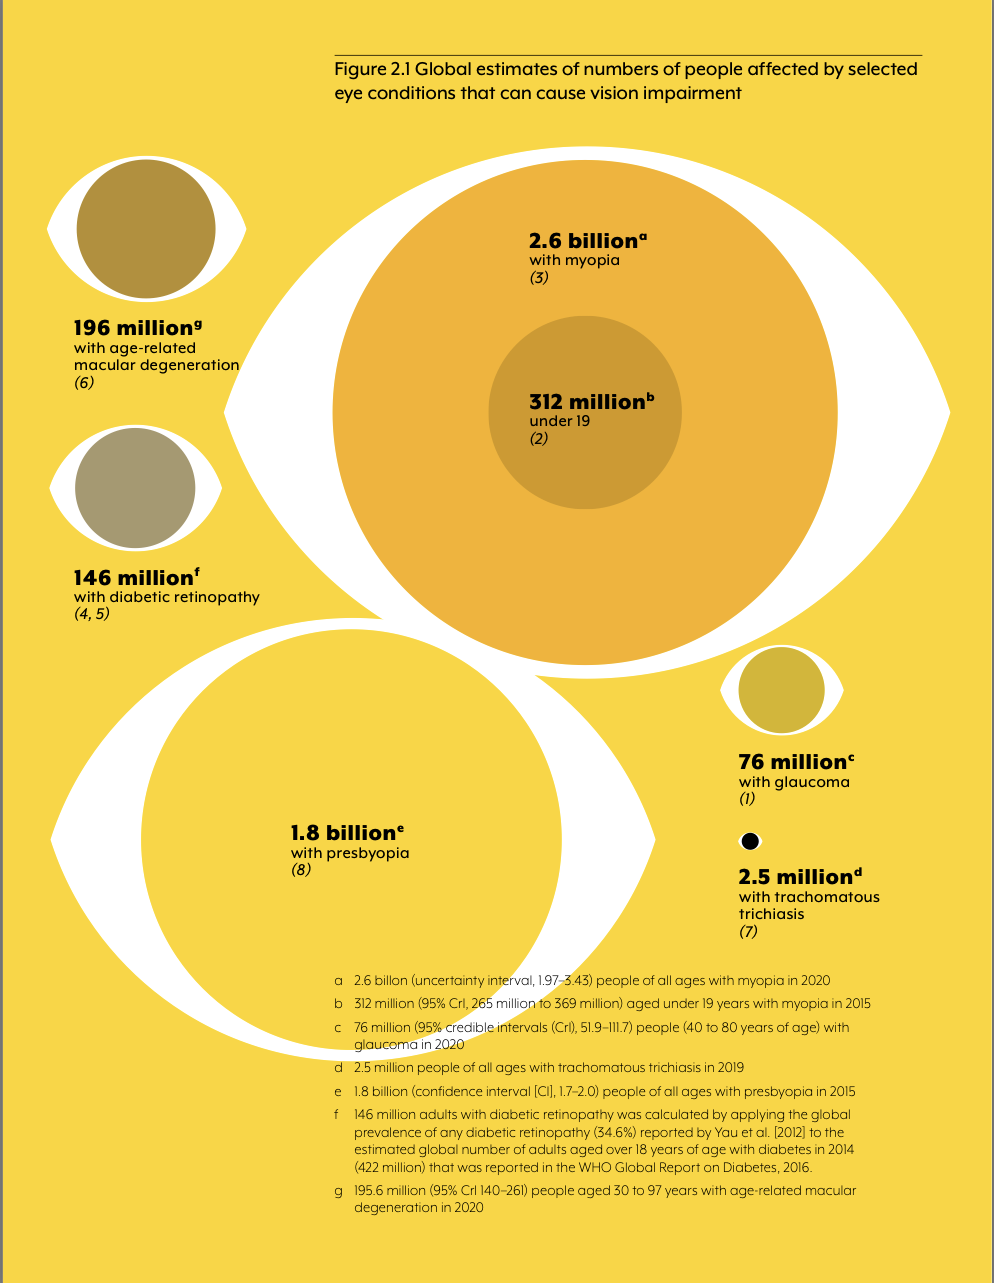
\includegraphics[width=\textwidth,height=0.75\textheight,keepaspectratio]{assets/global_eye_conditions.png}
    \caption{Global estimates of the number of people affected by major eye conditions causing vision impairment}
    \label{fig:global_eye_conditions}
\end{figure}

\newpage
\begin{figure}[H]
    \centering
    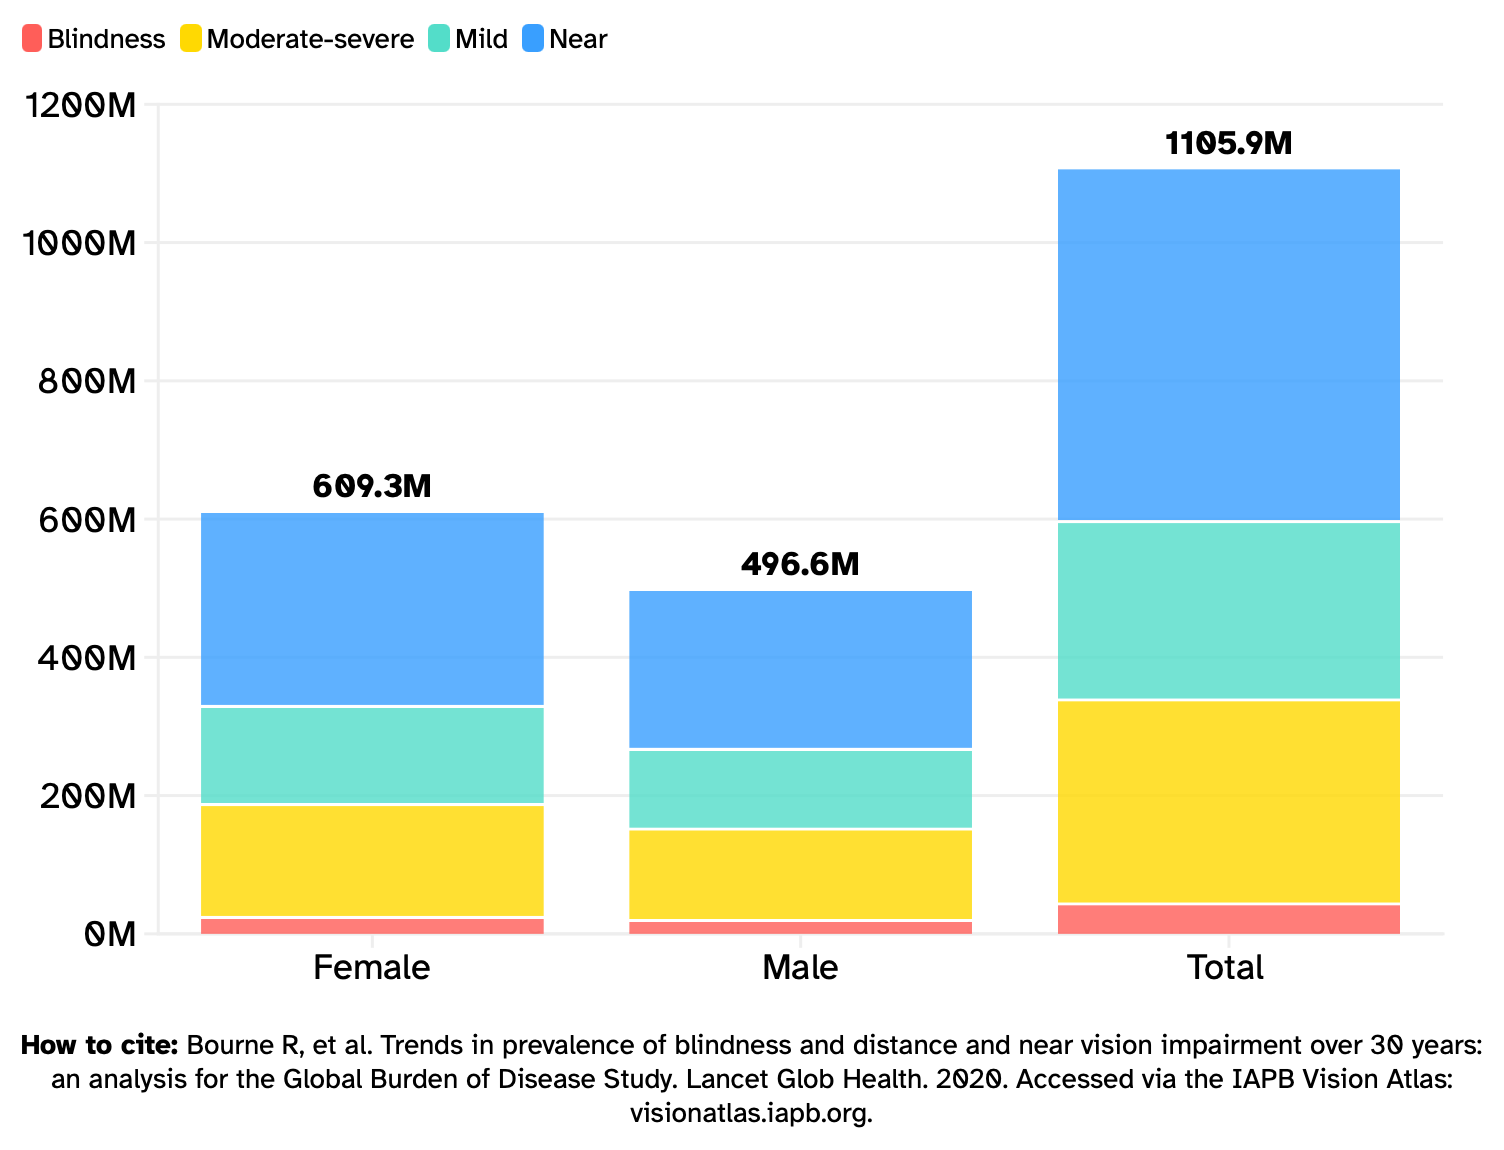
\includegraphics[width=0.8\textwidth]{assets/Worldwide analysis.png}
    \hfill
    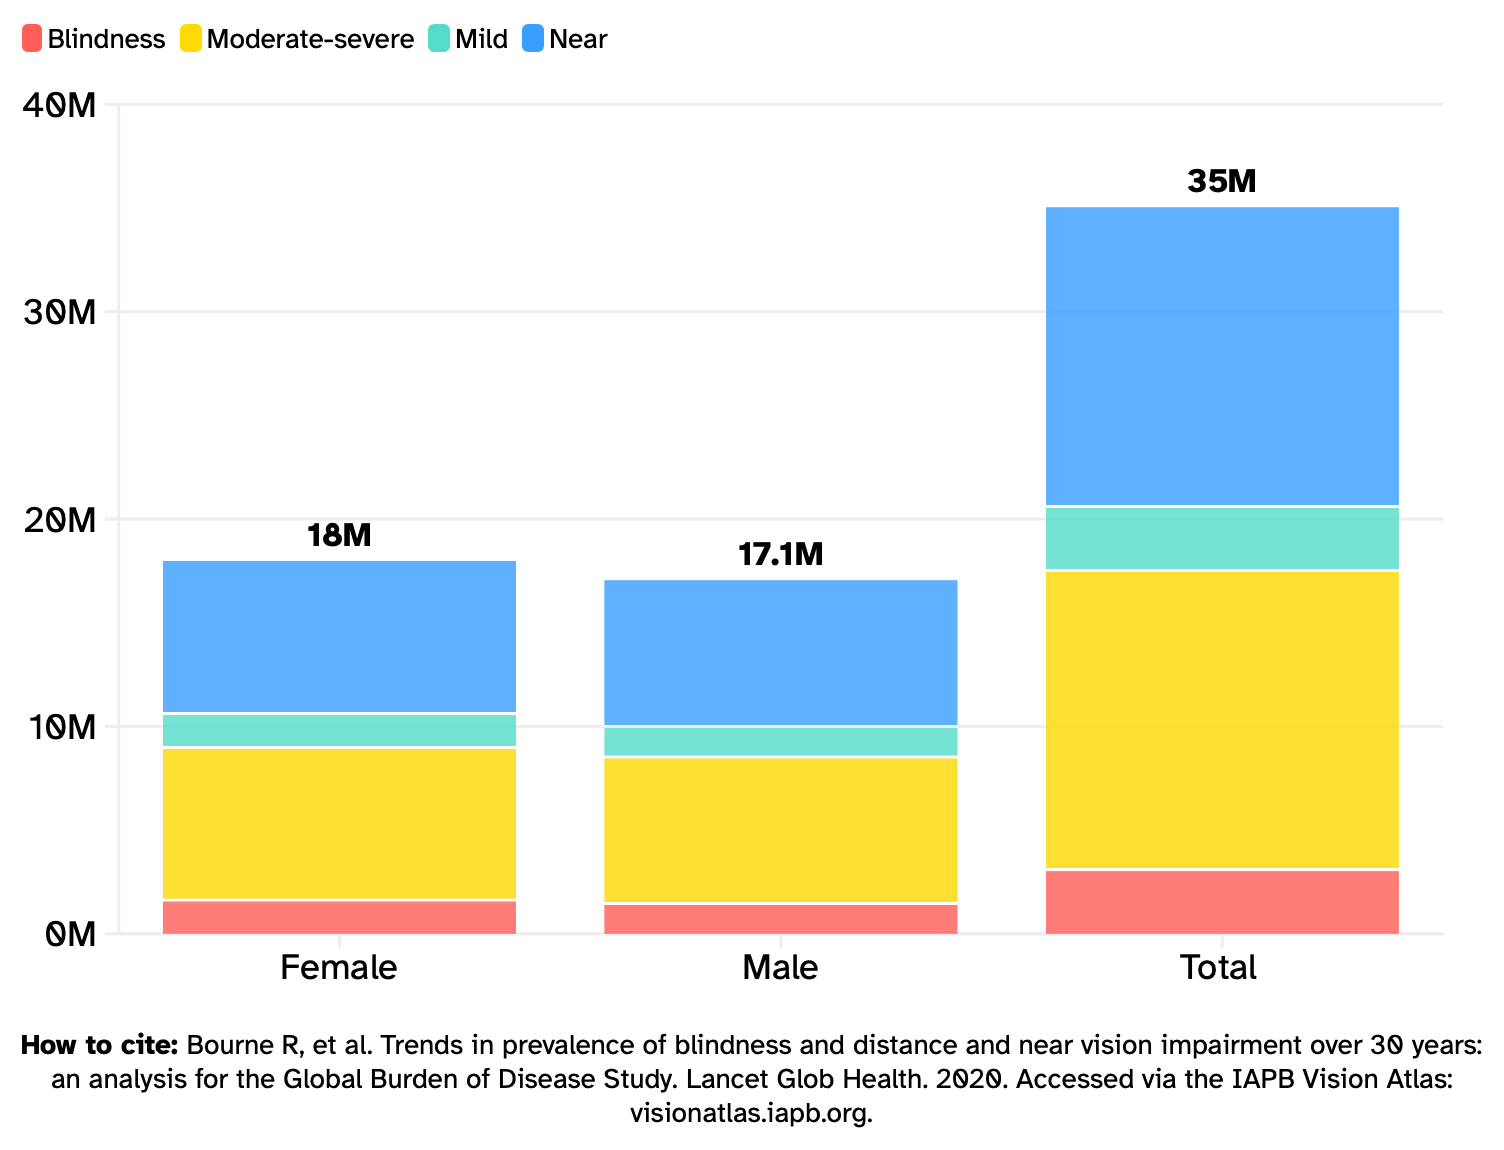
\includegraphics[width=0.8\textwidth]{assets/MiddlEeast analysis.png}
    \caption{Numbers of BLV population Worldwide and Middle East}
    \label{wor_mid_fig:blv_qol}
\end{figure}

\begin{figure}[H]
    \centering
    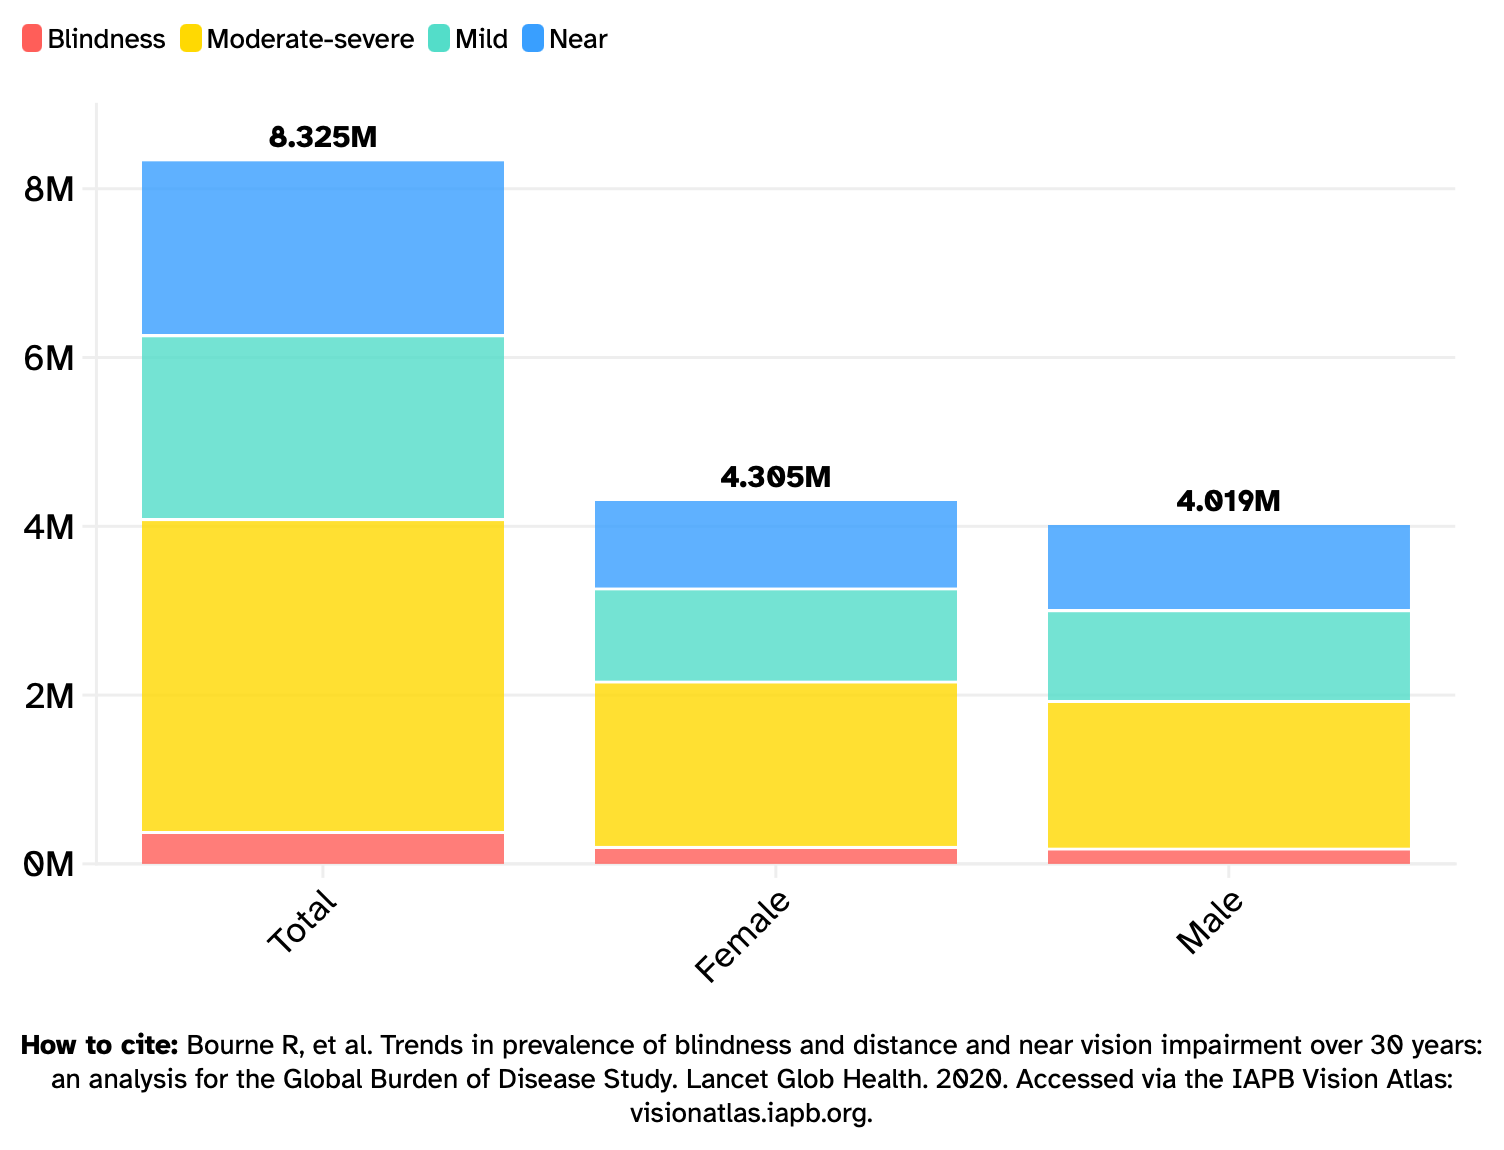
\includegraphics[width=0.7\textwidth]{assets/Egypt analysis.png}
    \caption{Numbers of BLV population in Egypt}
    \label{fig:eg_blv_qol}
\end{figure}

\begin{figure}[H]
    \centering
    
\includegraphics[width=\textwidth,height=0.75\textheight,keepaspectratio]{assets/sight-loss-over-time Egypt.png}
    \caption{Sight loss over time in Egypt}
    \label{fig:eg_sight_lossl}
\end{figure}

\begin{figure}[H]
    \centering
    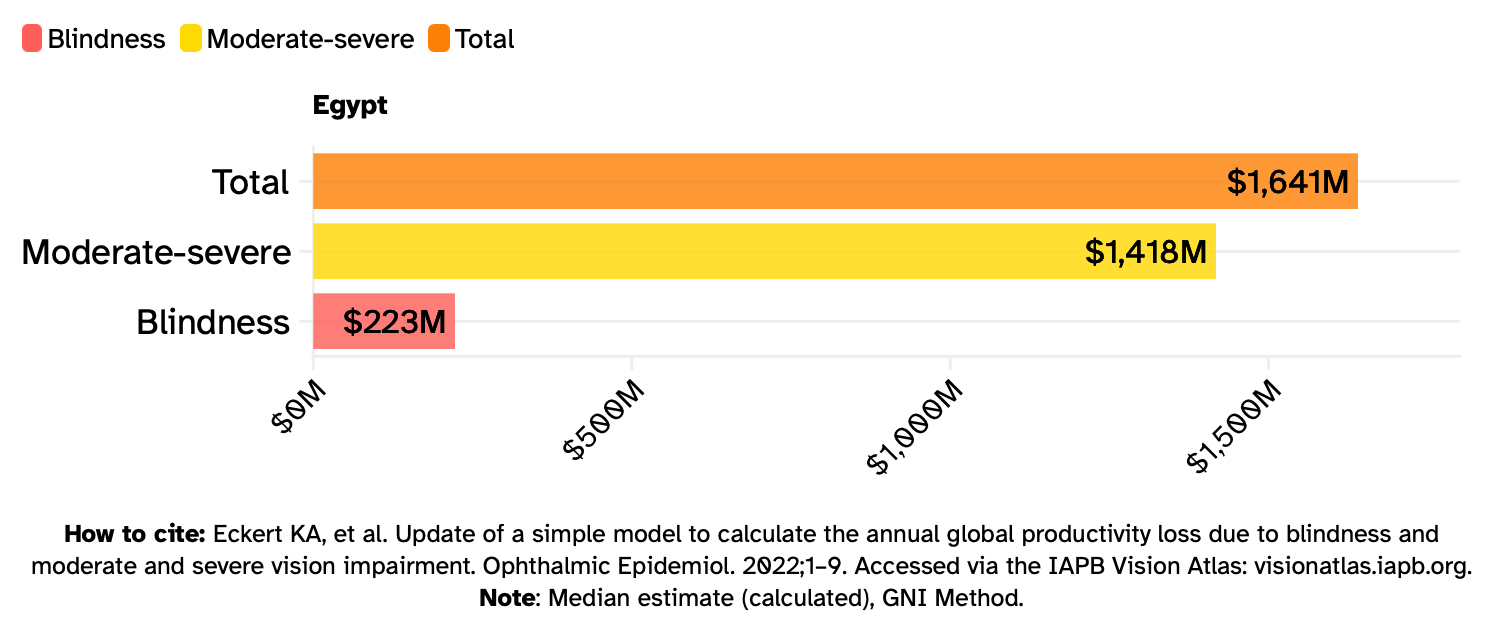
\includegraphics[width=\textwidth,height=0.75\textheight,keepaspectratio]{assets/productivity loss due to poor vision per year.png}
    \caption{Productivity loss due to poor vision per year in Egypt}
    \label{fig:lossl_per_year}
\end{figure}

\newpage
\section{Document Conventions}

This document follows a set of conventions to ensure clarity, consistency, and ease of understanding throughout the specification. These conventions define how terminology, requirements, and formatting are presented to maintain a professional and structured technical document.

\subsection{Typography Conventions}

Bold text is used to highlight key terms, feature names, and section headings upon their first occurrence in the document. Italic text is applied for emphasis and for introducing important concepts that require special attention. Monospace text is reserved for technical commands, code references, system identifiers, and system-generated messages. Functional requirements are numbered using the format FRX.Y, where X represents the feature number and Y represents the specific requirement within that feature.

\subsection{Requirement Priority Levels}

Requirements in this document are categorized based on their importance to system functionality and user safety. Critical (Live) requirements represent essential features that must be implemented to ensure core system operation and protect the user. High-priority requirements significantly enhance system performance and user experience but are not strictly mandatory for basic operation. Medium-priority requirements provide extended or optional functionality that may be included in later development stages.

\subsection{Stimulus-Response Format}

Functional requirements are specified using a stimulus-response format to clearly define system behavior. Each requirement describes a stimulus, which represents an event, input, or condition that triggers system behavior, followed by a response, which defines the expected system output or action resulting from that stimulus. This format supports clear validation and traceability of system behavior.

\section{Intended Audience}

This document is intended for multiple stakeholder groups involved in the development, evaluation, and understanding of the Echora system.

\subsection{Primary Audience}
\label{subsubsec:primary_audience}

The primary audience includes project developers and system designers responsible for implementing the Echora system, as well as testers and evaluators tasked with validating functional and non-functional requirements. It also serves as a reference for team members throughout the development lifecycle to ensure alignment with project objectives and specifications.

\subsection{Secondary Audience}
\label{subsubsec:secondary_audience}

The secondary audience consists of course instructors and academic supervisors overseeing the project, in addition to reviewers and evaluators assessing the project’s feasibility, technical correctness, and scope.

\subsection{Tertiary Audience}
\label{subsubsec:tertiary_audience}

The tertiary audience includes researchers and students interested in assistive technologies and sensory substitution systems, accessibility advocates, potential collaborators seeking an overview of the project, and readers with a general interest in AI-powered wearable assistive solutions.

\section{Project Scope}

This section defines the scope of the Echora project by outlining system boundaries, architectural assumptions, included features, excluded items, and supported Sustainable Development Goals.

\subsection{System Architecture}
\label{subsubsec:system_architecture}

The Echora system follows a distributed architecture that separates sensing and actuation from computation and intelligence. The architecture is composed of two main components: wearable hardware and PC-based processing software.

The wearable system consists of smart glasses equipped with a depth camera for environmental sensing, haptic actuators positioned on the wrist to deliver tactile feedback, a low-power microcontroller responsible for sensor data acquisition and communication, and a rechargeable battery that powers the wearable components. These hardware elements are designed exclusively for sensing and feedback purposes, with no artificial intelligence or high-level decision-making performed on the wearable device itself.

The PC-based processing software serves as the central processing unit of the system. It performs real-time processing of depth and visual data, executes artificial intelligence models for visual perception, object detection, hand tracking, and semantic understanding, manages interaction logic and automatic mode switching between recognition and interaction, generates audio feedback, and issues haptic control commands to the wearable device. This separation allows the wearable hardware to remain lightweight while enabling scalable software upgrades without requiring hardware modifications.

\subsection{Communication Protocol}
\label{subsubsec:communication_protocol}

The Echora system employs wireless communication to support real-time data exchange between the wearable hardware and the PC processing software. The communication design prioritizes low latency, reliability, and power efficiency to support continuous operation.

The wearable haptic module communicates with the PC over Wi-Fi. The module exposes a lightweight network interface around its ESP32 controller, and the PC sends it control instructions --- haptic feedback commands (direction, intensity, and confirmation patterns), mode changes, and warning signals --- in real time. High-bandwidth visual and depth data are handled on the PC directly from the OAK-D camera, so the wireless link carries only compact, low-latency control messages. All communication is designed to operate with minimal delay to ensure responsive and reliable user feedback.

\subsection{In-Scope Features}
\label{subsubsec:in_scope_features}

The scope of the Echora project includes real-time object awareness enabled through depth sensing, audio-based spatial feedback for interaction assistance, and haptic feedback for interaction safety and hand guidance. The system also supports object and interaction target detection, such as handles, buttons, and readable labels, as well as automatic switching between recognition and interaction modes based on user context.

\subsection{Out-of-Scope Items}
\label{subsubsec:out_of_scope}

The project explicitly excludes the replacement of traditional assistive tools such as white canes or guide dogs. It does not support autonomous recognition or decision-making without user control, nor does it provide medical diagnosis or treatment functionality. Cloud-based processing and continuous internet dependency are excluded to ensure offline usability. Additionally, the project does not include long-term user training or rehabilitation programs.

\subsection{Supported Sustainable Development Goals (SDGs)}
\label{subsubsec:sdgs}

The Echora project supports several United Nations Sustainable Development Goals. It contributes to SDG~3 by enhancing safety, independence, and quality of life for Blind and Low Vision users. It aligns with SDG~9 through the application of innovative AI and wearable technologies in assistive systems. The project promotes SDG~10 by reducing inequalities through improved access to recognition and interaction in physical environments. Finally, it supports SDG~11 by enabling inclusive and accessible urban daily interaction without requiring changes to existing infrastructure.

\section{Objectives}
\label{subsec:objectives}

The objectives of the Echora project define the intended outcomes and guide the design and development process. The system aims to enhance object awareness by providing continuous real-time perception of surrounding spaces, support safe recognition in indoor and outdoor environments, and enable precise object interaction by guiding the user’s hand toward interaction targets. It seeks to integrate multimodal sensor data into a unified perception model and deliver intuitive audio and haptic feedback that is easy to interpret. The project emphasizes minimizing cognitive load through context-aware adaptation, ensuring real-time performance with low latency, and leveraging PC computing to reduce hardware cost and improve scalability. The system is designed to maintain modularity for future extensions, complement existing assistive tools rather than replace them, and ultimately promote user independence and confidence.

\section{Challenges}
\label{subsec:challenges}

The development of the Echora system involves several technical, ethical, resource-related, and user experience challenges.

\subsection{Technical Challenges}
\label{subsubsec:technical_challenges}

From a technical perspective, the system must process multimodal sensor data in real time with minimal latency to ensure timely feedback. Sensor reliability remains a concern, as depth sensing and hand tracking accuracy can degrade in varying lighting conditions or cluttered environments. Designing effective audio and haptic feedback requires balancing informativeness with simplicity to avoid overwhelming the user. Wireless communication stability between wearable hardware and the PC is critical for responsiveness, and computational constraints on PCs may limit the simultaneous execution of multiple AI models.

\subsection{Ethical Challenges}
\label{subsubsec:ethical_challenges}

Ethical challenges include ensuring user privacy, particularly when camera and sensor data are collected from personal and public environments. The use of face recognition or individual identification requires careful consideration of consent and ethical boundaries. There is also a risk of user dependency if over-reliance on the system reduces situational awareness in the event of system failure. Maintaining user autonomy is essential, ensuring that the system assists rather than enforces actions.

\subsection{Resource-Related Challenges}
\label{subsubsec:resource_challenges}

Resource-related challenges arise from limited development time, which may restrict extensive testing and optimization. Hardware availability can be constrained by cost and supply limitations, and continuous sensing and processing can significantly impact battery life during prolonged use.

\subsection{User Experience Challenges}
\label{subsubsec:ux_challenges}

From a user experience perspective, learnability remains a key challenge, as users may require time to adapt to new audio and haptic cues. Cognitive load must be carefully managed to prevent information overload, and wearable components must remain comfortable and unobtrusive to support extended everyday use.

\newpage
\section{Risks}

\begin{table}[H]
\centering

\includegraphics[width=\textwidth]{assets/Risks.jpg}
\caption{List of Risks}
\label{tab:risks}
\end{table}

\newpage
\section{Standards}

\begin{table}[H]
\centering
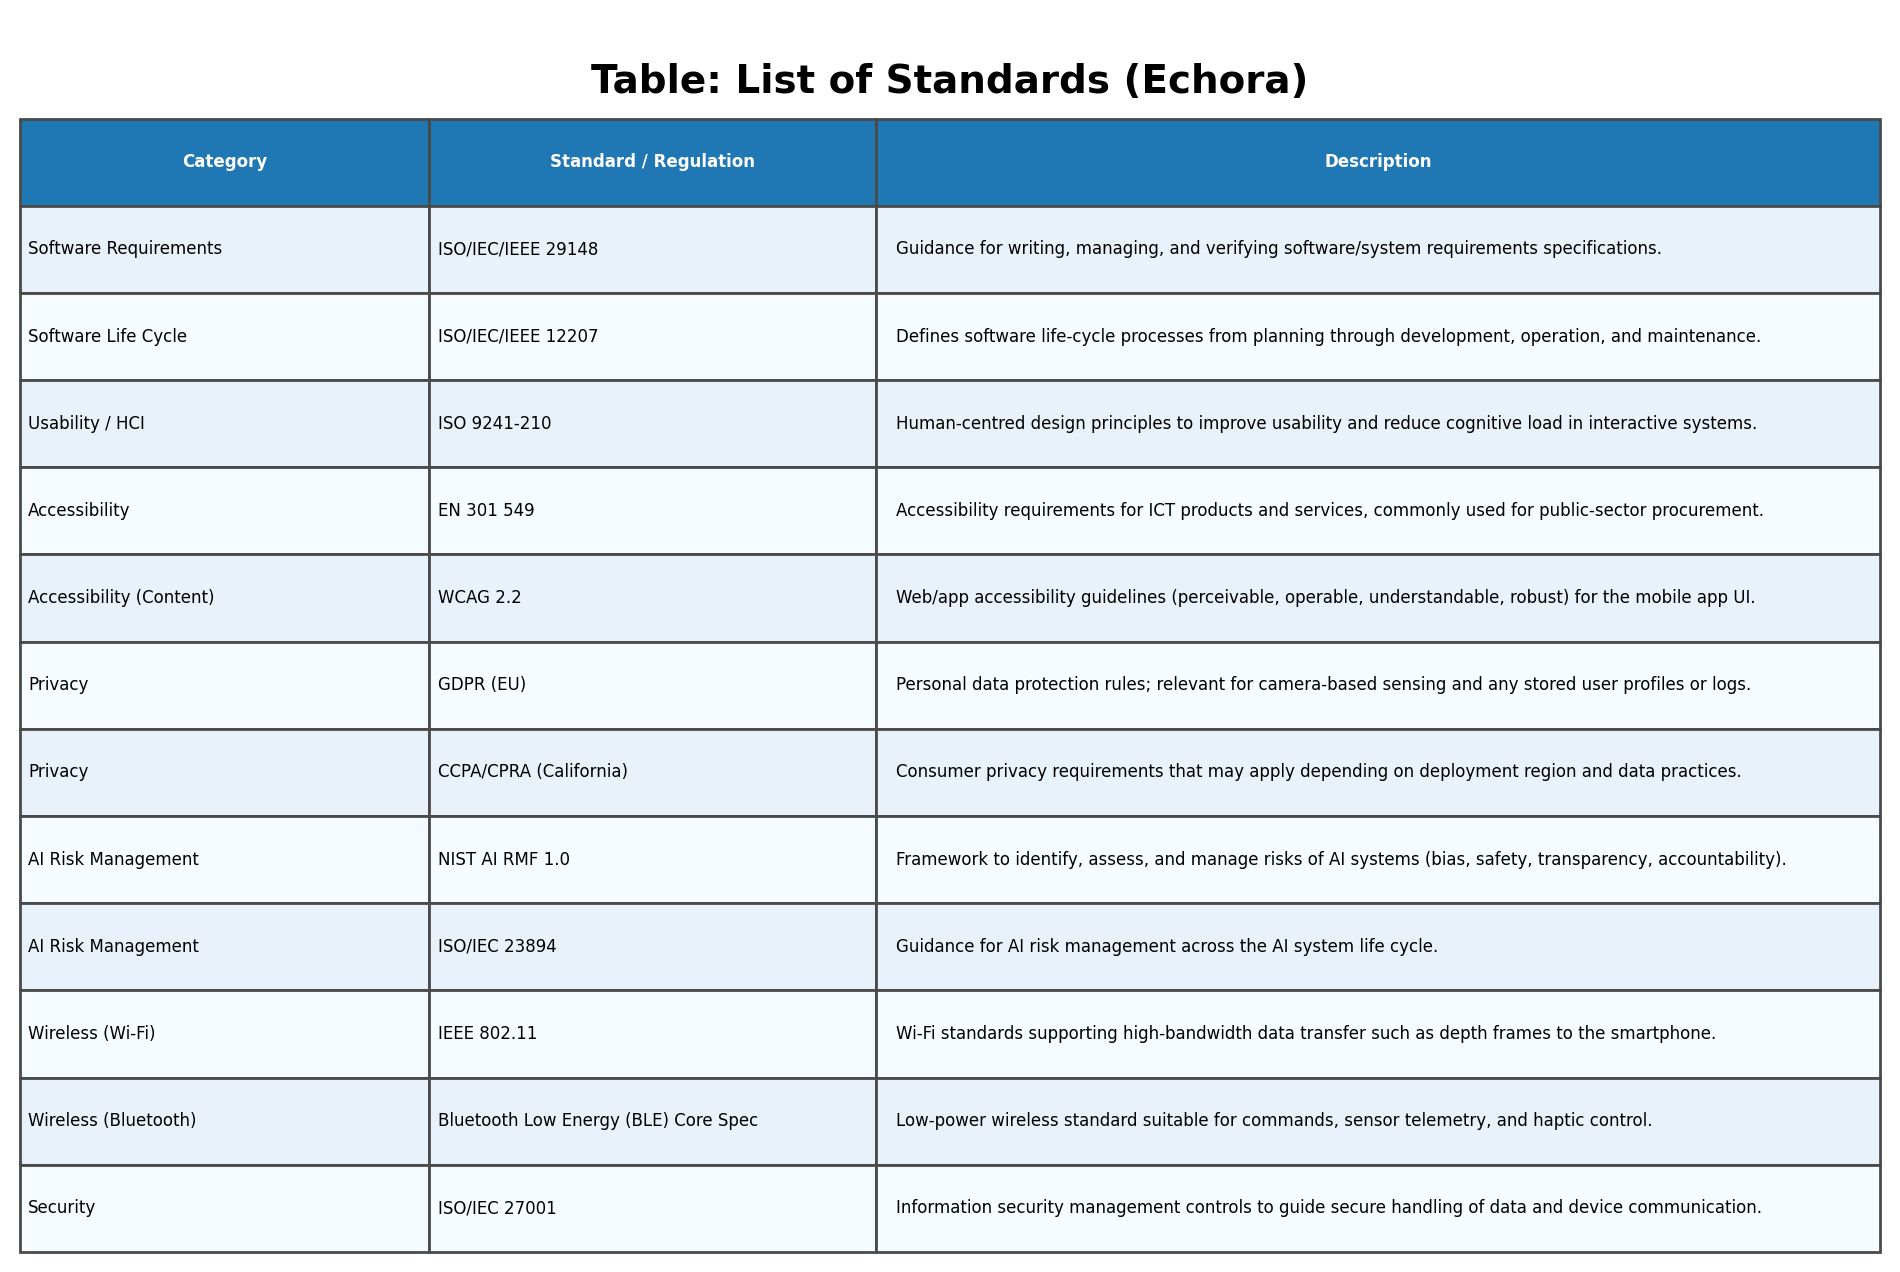
\includegraphics[width=\textwidth,height=0.75\textheight,keepaspectratio]{assets/echora_standards_table.png}
\caption{List of Standards}
\label{tab:standards}
\end{table}

\newpage
\section{Constraints}

\begin{table}[H]
\centering

\includegraphics[width=\textwidth,height=0.75\textheight,keepaspectratio]{assets/Constraints.jpg}
\caption{List of Constraints}
\label{tab:constraints}
\end{table}

\section{Summary}

This chapter introduced the Echora project and established the foundation for the remainder of the document. It outlined the purpose, intended use, and scope of the system, identifying the key challenges faced by Blind and Low Vision users in recognition and object interaction. The chapter also described the project’s objectives, system architecture overview, communication approach, and operational constraints.

In addition, potential challenges, risks, applicable standards, and constraints were discussed to highlight technical, ethical, and practical considerations influencing system design and development. Together, these elements define the problem space and clarify the boundaries within which Echora is developed.

The following chapter presents a detailed market analysis and review of related work, situating Echora within the broader context of existing assistive technologies and research efforts.
